\documentclass[letterpaper,10pt]{article}
\usepackage[top=2cm, bottom=1.5cm, left=1cm, right=1cm]{geometry}
\usepackage{amsmath, amssymb, amsthm,graphicx}
\usepackage{fancyhdr}
\pagestyle{fancy}

\lhead{\today}
\chead{Logistic Growth}
\rhead{Justin Hood}

\newcommand{\Z}{\mathbb{Z}}
\newcommand{\Q}{\mathbb{Q}}
\newcommand{\R}{\mathbb{R}}
\newcommand{\C}{\mathbb{C}}
\newtheorem{lem}{Lemma}
\title{Logistic Growth}
\author{Justin Hood\\
MATH 710\\
Dr. Wojciechowski}
\begin{document}
\maketitle
\newpage
We consider an equation describing Logarithmic Growth of a population with periodic harvesting from the population, based on the population size. Such an equation is,
\[\frac{dx}{dt}=s\bigg(1-\frac{x}{K}\bigg)x-hx\]
With $s$ being a ``rate constant", $K$ being the carrying capacity of the environment, and $h$ a unitless ``percentage" describing the harvesting from the population.\\
For the purposes of this analysis, we consider a population of deer, with starting population $900,000$. The habitat that the deer live in has a capacity of $1,072,764$. A suitable rate constant for this population of deer is $.2311$.\\
Let us now consider the effects of different harvesting terms on the overall behavior of the population. Starting at $1\%$ and increasing incrementally, we see that the harvesting term reduces the equilibrium behavior of the system. Consider below two examples with $h=.01$ on the left, and $h=.04$ on the right.\\
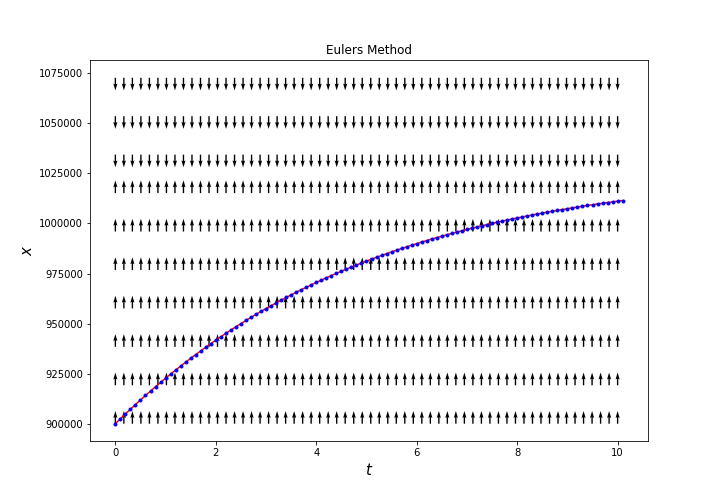
\includegraphics[scale=.4]{3a1.png}
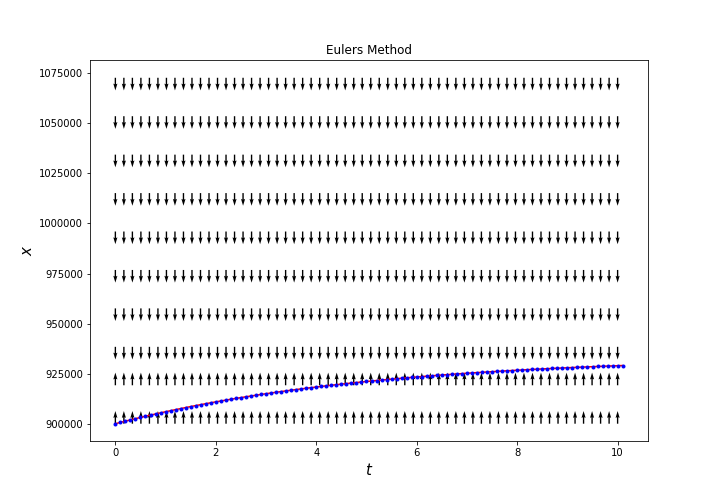
\includegraphics[scale=.4]{3a4.png}
We see that the solution curve with the higher harvesting rate has a lower long term population value. This leads to the obvious question, what are the equilibrium points of this model? As we have in the past, we shall set the differential equation equal to zero, and solve for $x$,
\begin{align*}
s(1-\frac{x}{K})x-hx &= 0\\
(s-h)x-\frac{s}{K}x^2 &= 0
\end{align*}
Substituting into the quadratic equation, we find the roots to be,
\[x=0,\ \frac{K(s-h)}{s}\]
So, the equilibrium points are zero, and a function of the constants in the differential equation. Considering the form of the non-zero equilibrium point, we note that as $h\to s$, the value of the equilibrium point will tend to zero. From this analysis, we may conclude that so long as $h<s$, the population will always tend towards a non-zero equilibrium point as defined by the root above. Should $h\geq s$, the population will decrease until it reaches extinction. To test this theory, we shall simulate the numeric solutions using the aforementioned constants $s$ and $K$, along with $h=\frac{s}{2},\text{and }h=s$. The plots follow.\\
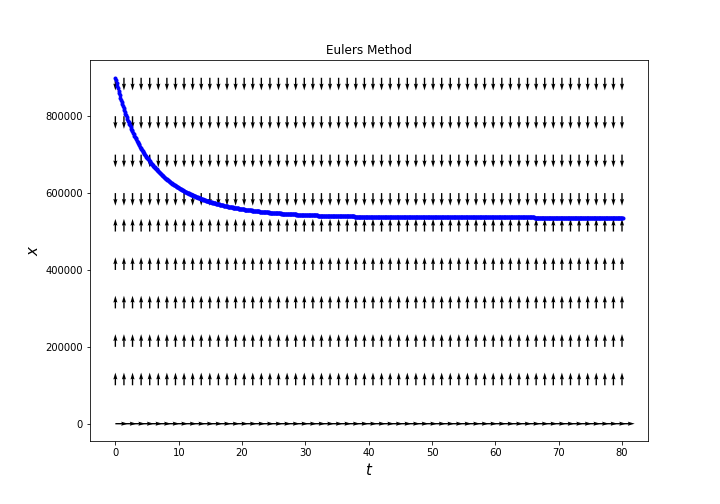
\includegraphics[scale=.4]{4b1.png}
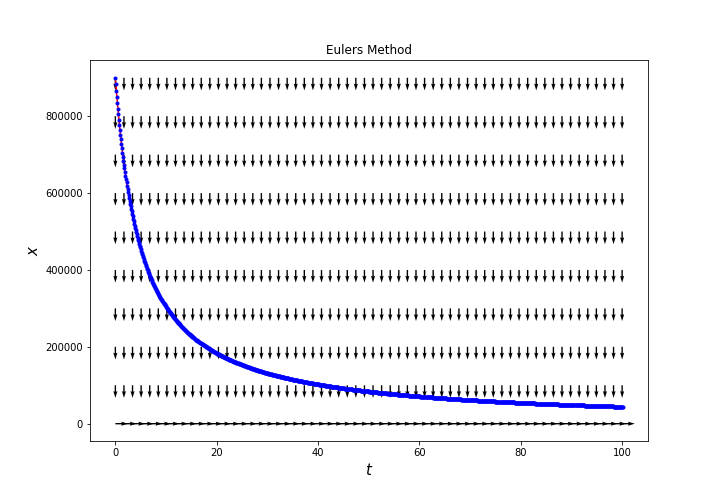
\includegraphics[scale=.4]{4b2.png}
On the left, we have $h=\frac{s}{2}$, and the right, $h=s$. As suggested by our analysis, the solution that tends to zero is the equation with $h=s$. It is worth noting as a point of curiosity that the solution with $h=\frac{s}{2}$ reaches a steady state at $\frac{K}{2}$.\\
Using this newfound knowledge of the effect of $h$ on the equilibrium populatiion value, we consider a situation wherein the population of deer needs to be controlled at a value lower than that of the carrying capacity of the environment itself. For instance, if the DNR wanted to maintain the deer population at $500,000$ in an effort to reduce disease spread and destruction of the habitat, they would need to hunt a certain amount of the deer each year. In order to compute this hunting constant, we consider the following.\\
As previously described, we know that the ending equilibrium population is directly affected by $h$. As we have fixed both $s$ and $K$, we may solve the following relation to arrive at the critical $h$ value.
\begin{align*}
500000 &= \frac{K(s-h^*)}{s}\\
500000s &= Ks-Kh^*\\
Kh^* &= Ks-500000s\\
h^* &= \frac{Ks-500000s}{K}
\end{align*}
Substituting in the values of $s$ and $K$, we arrive at,
\[h^*=.123388\]
Thus, we see that the optimal harvesting rate is $\approx12.339\%$. So, the DNR would need to cull a little over $12\%$ of the deer population each year in order to keep the population on track to equilibrate at $500000$.
\newpage
Note: All associated python files are included, with appropriate commenting for further experimentation.
\end{document}
